\begin{center}
	\Huge
	Variabeltransformation
\end{center}

\section*{Linearisering}
\stepcounter{section}

Vi husker os selv på, at forskriften for en eksponentialfunktion $f$ er givet ved
\begin{align*}
	f(x) = b\cdot a^x.
\end{align*}
Det viser sig, at vi kan lave grafen for $f$ til en ret linje ved at betragte et koordinatsystem med en sædvanlig $x$-akse og en $y$-akse, hvor vi har tallene $\log_{10}(y)$ i stedet for $y$. Et sådant koordinatsystem kaldes for et \textit{enkeltlogaritmisk koordinatsystem}. Hvilken logaritme, der anvendes er i vores sammenhæng underordnet.
\begin{setn}
	Grafen for funktionen $f$ givet ved
	\begin{align*}
		f(x) = b\cdot a^x
	\end{align*}
	vil være en ret linje i et enkeltlogaritmisk koordinatsystem.
\end{setn}
\begin{proof}
	Vi betragter udtrykket
	\begin{align*}
		y = b\cdot a^x.
	\end{align*}
	Vi tager $\log_{10}$ på begge sider af lighedstegnet og får
	\begin{align*}
		\log_{10}(y) &= \log_{10}(b\cdot a^x)\\
		&= \log_{10}(b) + \log_{10}(a^x)\\
		&= \log_{10}(b) + x\log_{10}(a).
	\end{align*}
	Der er altså en lineær sammenhæng mellem $x$ og $\log_{10}(y)$. 
\end{proof}

På Figur \ref{fig:exp} kan vi se grafen for funktionen $f$ givet ved
\begin{align*}
	f(x) = 2^x
\end{align*}
i et sædvanligt koordinatsystem og på Figur \ref{fig:linexp} kan vi se grafen for $f$ i et enkeltlogaritmisk koordinatsystem.
\begin{figure}[H]
	\centering
	\begin{minipage}{0.48\textwidth}
	\centering
	\resizebox{0.95\textwidth}{!}{
	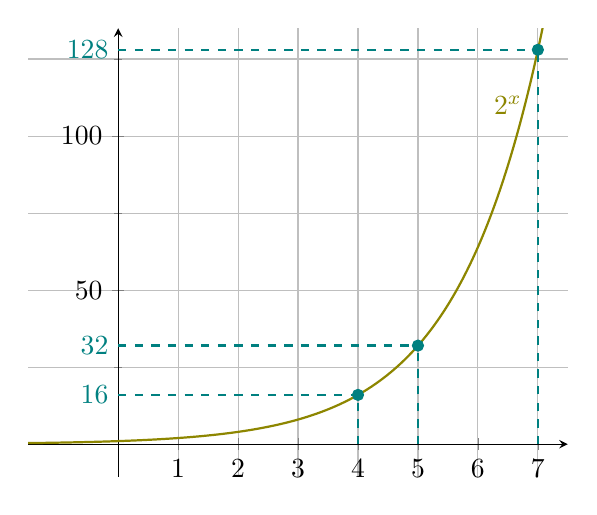
\begin{tikzpicture}
	\begin{axis}[
	axis lines = center, 
	xmin = -1.5, xmax = 7.5,
	ymin = -10.5, ymax = 135,
	xtick = {0,1,...,7,8},
	ytick = {-50,0,...,100,150},
	minor y tick num = 1,
	grid = both
	]
		
		\addplot[color = olive, thick, domain = -2:8, samples = 400] {2^x};

		\filldraw[color = teal] (axis cs: 4 , { 2^4 } ) circle (2pt);
		\draw[color = teal, dashed, thick] (axis cs: 4,0) -- (axis cs: 4, {2^4});
		\draw[color = teal, dashed, thick] (axis cs: 0,{2^4}) -- (axis cs: 4, {2^4});
		\node[anchor = east, color = teal] at (axis cs: 0,{2^4}) {$16$};
		\filldraw[color = teal] (axis cs: 5 , { 2^5 } ) circle (2pt);
		\draw[color = teal, dashed, thick] (axis cs: 5,0) -- (axis cs: 5, {2^5});
		\draw[color = teal, dashed, thick] (axis cs: 0,{2^5}) -- (axis cs: 5, {2^5});
		\node[anchor = east, color = teal] at (axis cs: 0,{2^5}) {$32$};
		\filldraw[color = teal] (axis cs: 7 , { 2^7 } ) circle (2pt);
		\draw[color = teal, dashed, thick] (axis cs: 7,0) -- (axis cs: 7, {2^7});
		\draw[color = teal, dashed, thick] (axis cs: 0,{2^7}) -- (axis cs: 7, {2^7});
		\node[anchor = east, color = teal] at (axis cs: 0,{2^7}) {$128$};
		\node[color = olive] at (axis cs: 6.5,110) {$2^x$};
	\end{axis}
	\end{tikzpicture}
	}
	\caption{Graf for funktionen $2^x$ i et sædvanligt koordinatsystem.}
	\label{fig:exp}
	\end{minipage}
	\begin{minipage}{0.48\textwidth}
	\centering
	\resizebox{0.95\textwidth}{!}{
	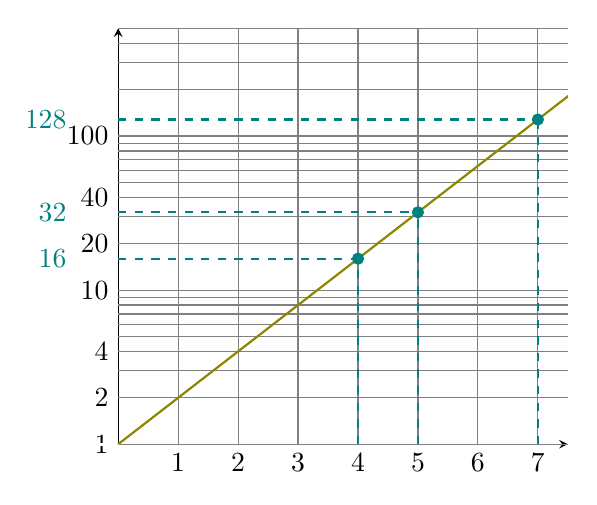
\begin{tikzpicture}
	\begin{axis}[
	axis lines = center, 
	xmin = -1.5, xmax = 7.5,
	ymin = -10.5, ymax = 135,
	ticks = none, 
	xlabel =
	]
		\pgfplotsinvokeforeach {1,...,10}
		{
		\draw[thin, color = gray] (axis cs: 0,{ 30.103/2*ln(#1)/ln(2) }) -- (axis cs: 8, { 30.103/2*ln(#1)/ln(2) });
		\draw[thin, color = gray] (axis cs: 0,{ 30.103/2*ln(#1)/ln(2) + 50 }) -- (axis cs: 8, { 30.103/2*ln(#1)/ln(2) + 50 });
		\draw[thin, color = gray] (axis cs: 0,{ 30.103/2*ln(#1)/ln(2) + 100 }) -- (axis cs: 8, { 30.103/2*ln(#1)/ln(2) + 100 });
		\draw[thin, color = gray] (axis cs: #1,0) -- (axis cs: #1,140);
		\node[anchor = north] at (axis cs: #1, 0) {$#1$};
		}
		\draw[color = white, very thick] (axis cs: 0,-30) -- (axis cs: 0,0);
		\pgfplotsinvokeforeach {1,2,4,10,20,40,100}
		{
		\node[anchor = east] at (axis cs: 0, { 30.103/2*ln(#1)/ln(2) }) {$#1$};
		}
		\addplot[color = white, very thick, domain = -5:0] {0}; 
		\draw[color = white, very thick] (axis cs: 0,-30) -- (axis cs: 0,0);
		\addplot[color = olive, thick, domain = 0:8] {15.052*x};
		\draw[color = teal, thick, dashed] (axis cs: 4,0) -- (axis cs: 4, 15.052*4);
		\draw[color = teal, thick, dashed] (axis cs: 5,0) -- (axis cs: 5, 15.052*5);
		\draw[color = teal, thick, dashed] (axis cs: 7,0) -- (axis cs: 7, 15.052*7);
		\filldraw[color = teal] (axis cs: 4, 15.052*4) circle (2pt);
		\filldraw[color = teal] (axis cs: 5, 15.052*5) circle (2pt);
		\filldraw[color = teal] (axis cs: 7, 15.052*7) circle (2pt);
		\draw[color = teal, thick, dashed] (axis cs: 0,15.052*4) -- (axis cs: 4, 15.052*4);
		\draw[color = teal, thick, dashed] (axis cs: 0,15.052*5) -- (axis cs: 5, 15.052*5);
		\draw[color = teal, thick, dashed] (axis cs: 0,15.052*7) -- (axis cs: 7, 15.052*7);
		\node[color = teal, anchor = east] at (axis cs: -0.7, 15.052*4) {$16$};
		\node[color = teal, anchor = east] at (axis cs: -0.7, 15.052*5) {$32$};
		\node[color = teal, anchor = east] at (axis cs: -0.7, 15.052*7) {$128$};
	\end{axis}
	\end{tikzpicture}
 	}
 	\caption{Graf for funktionen $2^x$ i et enkeltlogaritmisk koordinatsystem.}
 	\label{fig:linexp}
	\end{minipage}
\end{figure}

På samme måde som vi kan tegne en eksponentialfunktion som en ret linje i et enkeltlogaritmisk koordinatsystem kan vi tegne en potensfunktion som en ret linje i et \textit{dobbeltlogaritmisk koordinatsystem.} Et sådant koordinatsystem har akserne $\log_{10}(x)$ i stedet for $x$-aksen og $\log_{10}(y)$ i stedet for $y$-aksen. Igen er det ikke vigtigt, hvilken logaritme, vi bruger.
\begin{setn}
	Grafen for en potensfunktion $f$ givet ved
	\begin{align*}
		f(x) = b\cdot x^a
	\end{align*}
	er en ret linje i et dobbeltlogaritmisk koordinatsystem.
\end{setn}
\begin{proof}
	Vi har i en potenssammenhæng følgende sammenhæng mellem $x$ og $y$.
	\begin{align*}
		y = b\cdot x^a.
	\end{align*}
	Vi tager logaritmen på begge sider af lighedstegnet og får
	\begin{align*}
	 	\log_{10}(y) = \log_{10}(y \cdot x^a) \ &\Leftrightarrow \ \log_{10}(y) = \log_{10}(b) + 
	 	\log_{10}(x^a) \\
	 	&\Leftrightarrow	 \ \log_{10}(y) = \log_{10}(b) + a \log_{10}(x).
	\end{align*}
	Der er altså en lineær sammenhæng mellem $\log_{10}(y)$ og $\log_{10}(x)$.
\end{proof}
Vi kan på Figur \ref{fig:pow} se grafen for potensfunktionen $x^2$ i et sædvanligt koordinatsystem og på Figur \ref{fig:linpow} se grafen for $x^2$ i et dobbeltlogaritmisk koordinatsystem. 

\begin{figure}[H]
	\centering
	\begin{minipage}{0.48\textwidth}
	\centering
	\resizebox{0.95\textwidth}{!}{
	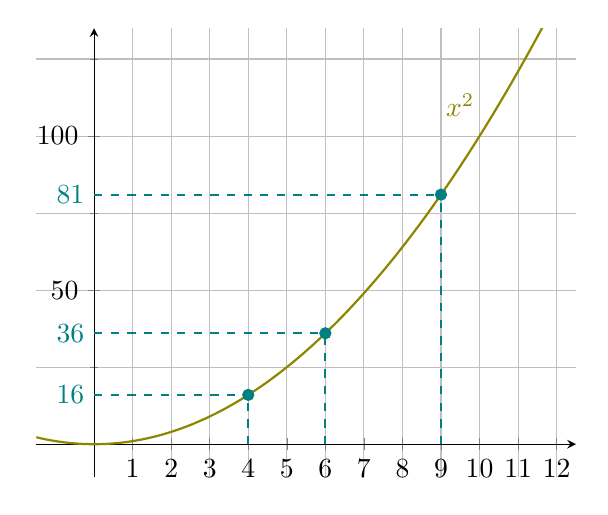
\begin{tikzpicture}
	\begin{axis}[
	axis lines = center, 
	xmin = -1.5, xmax = 12.5,
	ymin = -10.5, ymax = 135,
	xtick = {0,1,...,11,12},
	ytick = {-50,0,...,100,150},
	minor y tick num = 1,
	grid = both
	]
		
		\addplot[color = olive, thick, domain = -2:13, samples = 400] {x^2};

		\filldraw[color = teal] (axis cs: 4 , { 4^2 } ) circle (2pt);
		\draw[color = teal, dashed, thick] (axis cs: 4,0) -- (axis cs: 4, {4^2});
		\draw[color = teal, dashed, thick] (axis cs: 0,{4^2}) -- (axis cs: 4, {4^2});
		\node[anchor = east, color = teal] at (axis cs: 0,{4^2}) {$16$};
		\filldraw[color = teal] (axis cs: 6 , { 6^2 } ) circle (2pt);
		\draw[color = teal, dashed, thick] (axis cs: 6,0) -- (axis cs: 6, {6^2});
		\draw[color = teal, dashed, thick] (axis cs: 0,{6^2}) -- (axis cs: 6, {6^2});
		\node[anchor = east, color = teal] at (axis cs: 0,{6^2}) {$36$};
		\filldraw[color = teal] (axis cs: 9 , { 9^2 } ) circle (2pt);
		\draw[color = teal, dashed, thick] (axis cs: 9,0) -- (axis cs: 9, {9^2});
		\draw[color = teal, dashed, thick] (axis cs: 0,{9^2}) -- (axis cs: 9, {9^2});
		\node[anchor = east, color = teal] at (axis cs: 0,{9^2}) {$81$};
		\node[color = olive] at (axis cs: 9.5,110) {$x^2$};
	\end{axis}
	\end{tikzpicture}
	}
	\caption{Graf for funktionen $x^2$ i et sædvanligt koordinatsystem.}
	\label{fig:pow}
	\end{minipage}
	\begin{minipage}{0.48\textwidth}
	\centering
	\resizebox{0.95\textwidth}{!}{
	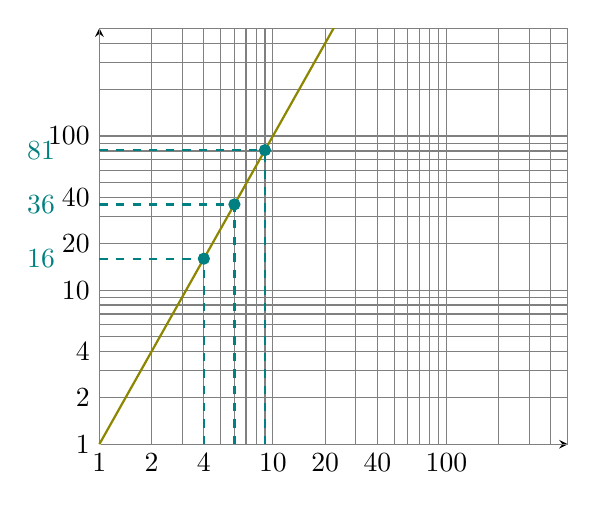
\begin{tikzpicture}
	\begin{axis}[
	axis lines = center, 
	xmin = -20.5, xmax = 135,
	ymin = -10.5, ymax = 135,
	ticks = none, 
	xlabel =
	]
		\pgfplotsinvokeforeach {1,...,10}
		{
		\draw[thin, color = gray] (axis cs: 0, { 30.103/2*ln(#1)/ln(2) }) -- (axis cs:150,  { 30.103/2*ln(#1)/ln(2) });
		\draw[thin, color = gray] (axis cs: 0,{ 30.103/2*ln(#1)/ln(2) + 50 }) -- (axis cs: 150 , { 30.103/2*ln(#1)/ln(2) + 50 });
		\draw[thin, color = gray] (axis cs: 0, { 30.103/2*ln(#1)/ln(2) + 100 }) -- (axis cs: 150, { 30.103/2*ln(#1)/ln(2) + 100 });
		\draw[thin, color = gray] (axis cs: { 30.103/2*ln(#1)/ln(2) }, 0) -- (axis cs:  { 30.103/2*ln(#1)/ln(2) }, 150);
		\draw[thin, color = gray] (axis cs: { 30.103/2*ln(#1)/ln(2) + 50 }, 0) -- (axis cs:  { 30.103/2*ln(#1)/ln(2) + 50 }, 150);
		\draw[thin, color = gray] (axis cs: { 30.103/2*ln(#1)/ln(2) + 100 }, 0) -- (axis cs:  { 30.103/2*ln(#1)/ln(2) + 100 }, 150);
		}
		\draw[color = white, very thick] (axis cs: 0,-30) -- (axis cs: 0,0);
		\addplot[color = white, very thick, domain = -50:0] {0}; 
		\draw[color = white, very thick] (axis cs: 0,-30) -- (axis cs: 0,0);
		\addplot[color = olive, thick, domain = 0:150] {2*x};
		\draw[color = teal, thick, dashed] (axis cs: {30.103/2*ln(4)/ln(2)},0) -- (axis cs: {30.103/2*ln(4)/ln(2)}, {30.103/2*2*ln(4)/ln(2)});
		\draw[color = teal, thick, dashed] (axis cs: {30.103/2*ln(6)/ln(2)},0) -- (axis cs: {30.103/2*ln(6)/ln(2)}, {30.103/2*2*ln(6)/ln(2)});
		\draw[color = teal, thick, dashed] (axis cs: {30.103/2*ln(9)/ln(2)},0) -- (axis cs: {30.103/2*ln(9)/ln(2)}, {30.103/2*2*ln(9)/ln(2)});
		\filldraw[color = teal] (axis cs: {30.103/2*ln(4)/ln(2)}, {2*30.103/2*ln(4)/ln(2)}) circle (2pt);
		\filldraw[color = teal] (axis cs: {30.103/2*ln(6)/ln(2)}, {2*30.103/2*ln(6)/ln(2)}) circle (2pt);
		\filldraw[color = teal] (axis cs: {30.103/2*ln(9)/ln(2)}, {2*30.103/2*ln(9)/ln(2)}) circle (2pt);
		\draw[color = teal, thick, dashed] (axis cs: 0,{2*30.103/2*ln(4)/ln(2)}) -- (axis cs: {30.103/2*ln(4)/ln(2)}, {2*30.103/2*ln(4)/ln(2)});
		\draw[color = teal, thick, dashed] (axis cs: 0,{2*30.103/2*ln(6)/ln(2)}) -- (axis cs: {30.103/2*ln(6)/ln(2)}, {2*30.103/2*ln(6)/ln(2)});
		\draw[color = teal, thick, dashed] (axis cs: 0,{2*30.103/2*ln(9)/ln(2)}) -- (axis cs: {30.103/2*ln(9)/ln(2)}, {2*30.103/2*ln(9)/ln(2)});
		\pgfplotsinvokeforeach {1,2,4,10,20,40,100}
		{
		\node[anchor = east] at (axis cs: 0, { 30.103/2*ln(#1)/ln(2) }) {$#1$};
		\node[anchor = north] at (axis cs: {30.103/2*ln(#1)/ln(2)}, 0) {$#1$};
		}
		\pgfplotsinvokeforeach {16,36,81}
		{
		\node[anchor = east, color = teal] at (axis cs: -10, { 30.103/2*ln(#1)/ln(2) }) {$#1$};
		}
	\end{axis}
	\end{tikzpicture}
 	}
 	\caption{Graf for funktionen $x^2$ i et dobbeltlogaritmisk koordinatsystem.}
 	\label{fig:linpow}
	\end{minipage}
\end{figure}

\subsection*{Opgave 1}
\begin{enumerate}[label=\roman*)]
	\item Tegn punkterne $(1,2)$ og $(4,16)$ ind på et enkeltlogaritmisk og forbind dem med en ret 
	linje.
	\item Brug linjen til at udfylde følgende tabel.
	\begin{center}
		\begin{tabular}{c|c|c|c|c|c|c|c|c|c|c}
			$x$ & 1 & 2 & 3 & 4 & 5 & 6 & 7 & 8 & 9 & 10 \\
			\hline
			$y$ & 2 & \phantom{4}  & \phantom{8}  &16 & \phantom{32}  & \phantom{64}  & \phantom{128}  & \phantom{256}  & \phantom{512}  & \phantom{1024}
		\end{tabular}
	\item Kan du gennemskue hvilken sammenhæng, linjen beskriver? (Vink: Overvej, hvad der sker med
	tallene, når $x$ øges med 1.)
	\end{center}
\end{enumerate}

\subsection*{Opgave 2}
\begin{enumerate}[label=\roman*)]
	\item Tegn punkterne $(2,18)$ og $(4,162)$ ind på et enkeltlogaritmisk koordinatsystem og forbind dem med en ret 
	linje.
	\item Brug linjen til at udfylde følgende tabel.
	\begin{center}
		\begin{tabular}{c|c|c|c|c|c}
			$x$ & 1 & 2 & 3 & 4 & 5  \\
			\hline
			$y$ & \phantom{6} & 18 & \phantom{54} & 162 & \phantom{486}
		\end{tabular}
	\end{center}
	\item Kan du gennemskue hvilken sammenhæng, linjen beskriver? 
\end{enumerate}

\subsection*{Opgave 3}

\begin{enumerate}[label=\roman*)]
	\item Grafen for en funktion $f$ er en ret linje i et enkeltlogaritmisk koordinatsystem. Grafen for $f$ går 
	gennem punkterne $(3,2)$ og $(6,16)$. Bestem en forskrift for $f$ uden at tegne grafen.
\end{enumerate}

\subsection*{Opgave 4}

\begin{enumerate}[label=\roman*)]
	\item Tegn punkterne $(2,4)$ og $(6,36)$ ind på et dobbeltlogaritmisk koordinatsystem og forbind dem med 
	en ret linje.
	\item Brug linjen til at udfylde følgende tabel.
	\begin{center}
		\begin{tabular}{c|c|c|c|c|c|c|c|c|c|c}
			$x$ & 1 & 2 & 3 & 4 & 5 & 6 & 10 & 20 & 40 & 80 \\
			\hline
			$y$ & \phantom{1} & 4  & \phantom{8}  &\phantom{16} & \phantom{32}  & 36  & \phantom{128}  & \phantom{256}  & \phantom{512}  & \phantom{1024}
		\end{tabular}
	\item Kan du gennemskue hvilken sammenhæng, linjen beskriver? 
	\end{center}
\end{enumerate}

\subsection*{Opgave 5}
\begin{enumerate}[label=\roman*)]
	\item Tegn punkterne $(1,2)$ og $(4,128)$ ind på et enkeltlogaritmisk koordinatsystem og forbind dem med en ret 
	linje.
	\item Brug linjen til at udfylde følgende tabel.
	\begin{center}
		\begin{tabular}{c|c|c|c|c|c|c}
			$x$ & 1 & 2 & 3 & 4 & 5 & 6  \\
			\hline
			$y$ & 2 & \phantom{18} & \phantom{54} & 162 & \phantom{486}& \phantom{600}
		\end{tabular}
	\end{center}
	\item Kan du gennemskue hvilken sammenhæng, linjen beskriver? 
\end{enumerate}

\subsection*{Opgave 6 (Med Maple)}
\begin{enumerate}[label=\roman*)]
	\item Grafen for en funktion $f$ er på et dobbeltlogaritmisk koordinatsystem en ret linje. Grafen for $f$
	går gennem punkterne $(5,9)$ og $(13,107)$. Bestem en forskrift for $f$ uden at tegne grafen. 
\end{enumerate}

\subsection*{Opgave 7}
Vi skal vise, at eksponentielle sammenhænge mellem to variable $x$ og $y$ vil være lineære på enkeltlogaritmisk papir. Vi husker os selv på, at en eksponentiel sammenhæng mellem to variable er på formen
\begin{align}
	\label{eq:exp}
	y = b\cdot a^x
\end{align}
\begin{enumerate}[label=\roman*)]
	\item Tag logaritmen på begge sider af lighedstegnet på \eqref{eq:exp}.
	\item Anvend to logaritmeregneregler på udtrykket.
	\item Er der en lineær sammenhæng mellem $x$ og $\log(y)$?
\end{enumerate}

\subsection*{Opgave 8}
Vi skal vise, at potenssammenhænge mellem to variable $x$ og $y$ vil være lineære på dobbeltlogaritmisk papir. Vi husker os selv på, at en potenssammenhæng mellem to variable er på formen
\begin{align}
	\label{eq:pow}
	y = b\cdot x^a
\end{align}
\begin{enumerate}[label=\roman*)]
	\item Tag logaritmen på begge sider af lighedstegnet på \eqref{eq:pow}.
	\item Anvend to logaritmeregneregler på udtrykket.
	\item Er der en lineær sammenhæng mellem $\log(x)$ og $\log(y)$?
\end{enumerate}

